\documentclass[12pt,a4paper]{scrartcl}\usepackage[]{graphicx}\usepackage[]{color}
% maxwidth is the original width if it is less than linewidth
% otherwise use linewidth (to make sure the graphics do not exceed the margin)
\makeatletter
\def\maxwidth{ %
  \ifdim\Gin@nat@width>\linewidth
    \linewidth
  \else
    \Gin@nat@width
  \fi
}
\makeatother

\definecolor{fgcolor}{rgb}{0.345, 0.345, 0.345}
\newcommand{\hlnum}[1]{\textcolor[rgb]{0.686,0.059,0.569}{#1}}%
\newcommand{\hlstr}[1]{\textcolor[rgb]{0.192,0.494,0.8}{#1}}%
\newcommand{\hlcom}[1]{\textcolor[rgb]{0.678,0.584,0.686}{\textit{#1}}}%
\newcommand{\hlopt}[1]{\textcolor[rgb]{0,0,0}{#1}}%
\newcommand{\hlstd}[1]{\textcolor[rgb]{0.345,0.345,0.345}{#1}}%
\newcommand{\hlkwa}[1]{\textcolor[rgb]{0.161,0.373,0.58}{\textbf{#1}}}%
\newcommand{\hlkwb}[1]{\textcolor[rgb]{0.69,0.353,0.396}{#1}}%
\newcommand{\hlkwc}[1]{\textcolor[rgb]{0.333,0.667,0.333}{#1}}%
\newcommand{\hlkwd}[1]{\textcolor[rgb]{0.737,0.353,0.396}{\textbf{#1}}}%
\let\hlipl\hlkwb

\usepackage{framed}
\makeatletter
\newenvironment{kframe}{%
 \def\at@end@of@kframe{}%
 \ifinner\ifhmode%
  \def\at@end@of@kframe{\end{minipage}}%
  \begin{minipage}{\columnwidth}%
 \fi\fi%
 \def\FrameCommand##1{\hskip\@totalleftmargin \hskip-\fboxsep
 \colorbox{shadecolor}{##1}\hskip-\fboxsep
     % There is no \\@totalrightmargin, so:
     \hskip-\linewidth \hskip-\@totalleftmargin \hskip\columnwidth}%
 \MakeFramed {\advance\hsize-\width
   \@totalleftmargin\z@ \linewidth\hsize
   \@setminipage}}%
 {\par\unskip\endMakeFramed%
 \at@end@of@kframe}
\makeatother

\definecolor{shadecolor}{rgb}{.97, .97, .97}
\definecolor{messagecolor}{rgb}{0, 0, 0}
\definecolor{warningcolor}{rgb}{1, 0, 1}
\definecolor{errorcolor}{rgb}{1, 0, 0}
\newenvironment{knitrout}{}{} % an empty environment to be redefined in TeX

\usepackage{alltt}
\usepackage[utf8]{inputenc}
\usepackage{amsmath}
\usepackage{graphicx}
\usepackage{tikz}
%\usepackage{silence}
\usepackage{mdframed}
%\WarningFilter{mdframed}{You got a bad break}
\usepackage[colorinlistoftodos]{todonotes}
\usepackage{listings}
\usepackage{color}
\colorlet{exampcol}{blue!10}
\usepackage{multicol}
\usepackage{booktabs}


\usepackage{tcolorbox}


\usepackage{setspace}
%\doublespacing

\usepackage[noanswer]{exercise}%[noanswer]
\renewcommand{\ExerciseHeaderTitle}{\quad---\quad \color{orange!70!black}\ExerciseTitle}


\usepackage[autostyle, english = american]{csquotes}
\MakeOuterQuote{"}

\usepackage{hyperref}
\hypersetup{
    colorlinks,
    citecolor=black,
    filecolor=black,
    linkcolor=blue,
    urlcolor=blue
}

\title{R-StatProgamming with functions in R}
\date{\today}
\author{Timoth\'ee Bonnet, BDSI}
\IfFileExists{upquote.sty}{\usepackage{upquote}}{}
\begin{document}



\maketitle

On Friday 03/04/2020 I will be presenting this tutorial live on Zoom. (ask by email/Slack if you do not know how to use Zoom.)

If you have any trouble going through this tutorial then or at a different time you can chat about it on Slack ( rsb-r-stats-biology.slack.com , if you are not a member but would like to be, drop me an email) or email me at \href{mailto:timotheebonnetc@gmail.com}{timotheebonnetc@gmail.com}.

If you do not attend the Zoom meeting but would like to receive credit through the \href{https://wattlecourses.anu.edu.au/enrol/index.php?id=23938}{COS Career Development Framework} program I need you to complete three exercises of your choice. Send me your answers via Slack or email. It does not have to be correct on the first try and you are welcome to get in touch if you are completely stuck. I will provide feedback to help you complete exercises you want to do.

In this tutorial you will learn:

\begin{itemize}
    \item How unexplained variation in a response variable can compromise statistical inference when that variation is structured.
    \item How fixed and random effects can correct for structured variation in the response variable.
    \item How to fit mixed-effects models in R.
    \item How to choose between fixed and random effects.
    \item Extract and interpret mixed models output.
\end{itemize}

\tableofcontents
\ListOfExerciseInToc
\ExerciseLevelInToc{subsubsection}

\clearpage

\section{The dangers of unexplained variation}
Imagine you have measured how much a plant species is attacked by big herbivores as a function of how many thorns the plant grows on stems. You have collected data in 5 locations and visualise the relationship between herbivory and quantity of thorns (in arbitrary units):
\begin{center}
  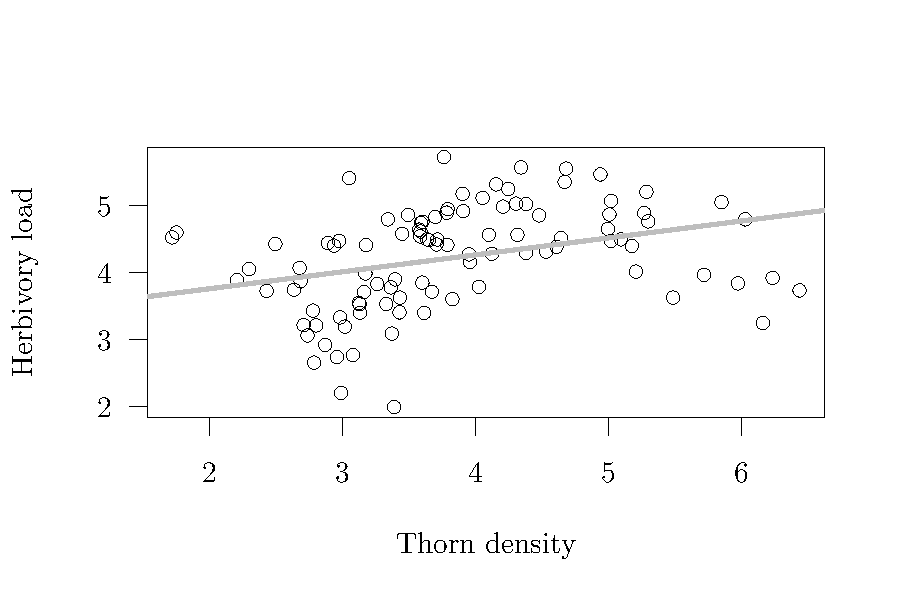
\includegraphics[width=0.8\textwidth]{figures/graph0-1.pdf}
\end{center}

It looks like the more a plant has thorns, the more it is eaten. Let's check that by fitting a linear regression.

\begin{knitrout}
\definecolor{shadecolor}{rgb}{0.969, 0.969, 0.969}\color{fgcolor}\begin{kframe}
\begin{alltt}
\hlstd{thorns} \hlkwb{<-} \hlkwd{read.csv}\hlstd{(}\hlkwc{file} \hlstd{=} \hlstr{"Data/thorndata.csv"}\hlstd{,} \hlkwc{header}\hlstd{=}\hlnum{TRUE}\hlstd{)}
\hlkwd{str}\hlstd{(thorns)}
\end{alltt}
\begin{verbatim}
## 'data.frame':	100 obs. of  3 variables:
##  $ herbivory   : num  4.53 4.6 3.89 4.05 3.73 ...
##  $ thorndensity: num  1.72 1.75 2.2 2.3 2.43 ...
##  $ site        : Factor w/ 5 levels "a","b","c","d",..: 1 1 1 1 1 1 1 1 1 1 ...
\end{verbatim}
\begin{alltt}
\hlstd{model_0} \hlkwb{<-} \hlkwd{lm}\hlstd{(herbivory} \hlopt{~} \hlstd{thorndensity,} \hlkwc{data} \hlstd{= thorns)}
\hlkwd{summary}\hlstd{(model_0)}
\end{alltt}
\begin{verbatim}
## 
## Call:
## lm(formula = herbivory ~ thorndensity, data = thorns)
## 
## Residuals:
##     Min      1Q  Median      3Q     Max 
## -2.1162 -0.5183  0.0821  0.5435  1.5193 
## 
## Coefficients:
##              Estimate Std. Error t value Pr(>|t|)    
## (Intercept)    3.2564     0.2854   11.41  < 2e-16 ***
## thorndensity   0.2524     0.0717    3.52  0.00066 ***
## ---
## Signif. codes:  0 '***' 0.001 '**' 0.01 '*' 0.05 '.' 0.1 ' ' 1
## 
## Residual standard error: 0.725 on 98 degrees of freedom
## Multiple R-squared:  0.112,	Adjusted R-squared:  0.103 
## F-statistic: 12.4 on 1 and 98 DF,  p-value: 0.000657
\end{verbatim}
\end{kframe}
\end{knitrout}
This model confirms a positive relationship between how much a plant has thorns and how much it is consumed by herbivores; which is counter-intuitive.

The twist is that data were collected in 5 different sites, that our two variables have different mean values in different sites, and that our model is not aware of that. 
We can see the structure in the data by coloring the points by site:
\begin{center}
  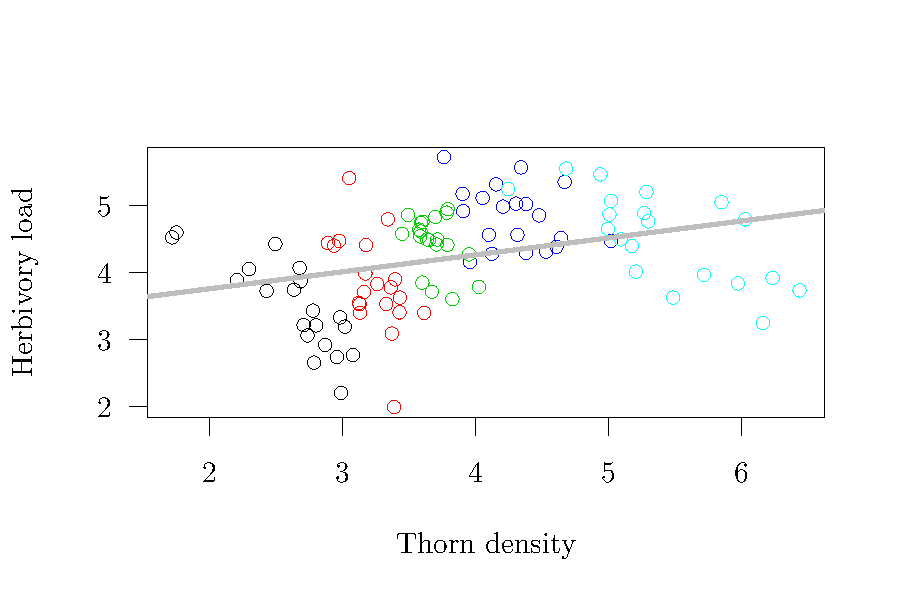
\includegraphics[width=0.8\textwidth]{figures/graph1-1.pdf}
\end{center}

Maybe you remember that in a linear model (such as a linear regression) we assume that the residuals follow a normal distribution without any structure (homoscedasticity, independence\dots).
It is not easy to see patterns by just ploting the residuals:
\begin{knitrout}
\definecolor{shadecolor}{rgb}{0.969, 0.969, 0.969}\color{fgcolor}\begin{kframe}
\begin{alltt}
\hlkwd{plot}\hlstd{(}\hlkwd{residuals}\hlstd{(model_0))}
\end{alltt}
\end{kframe}
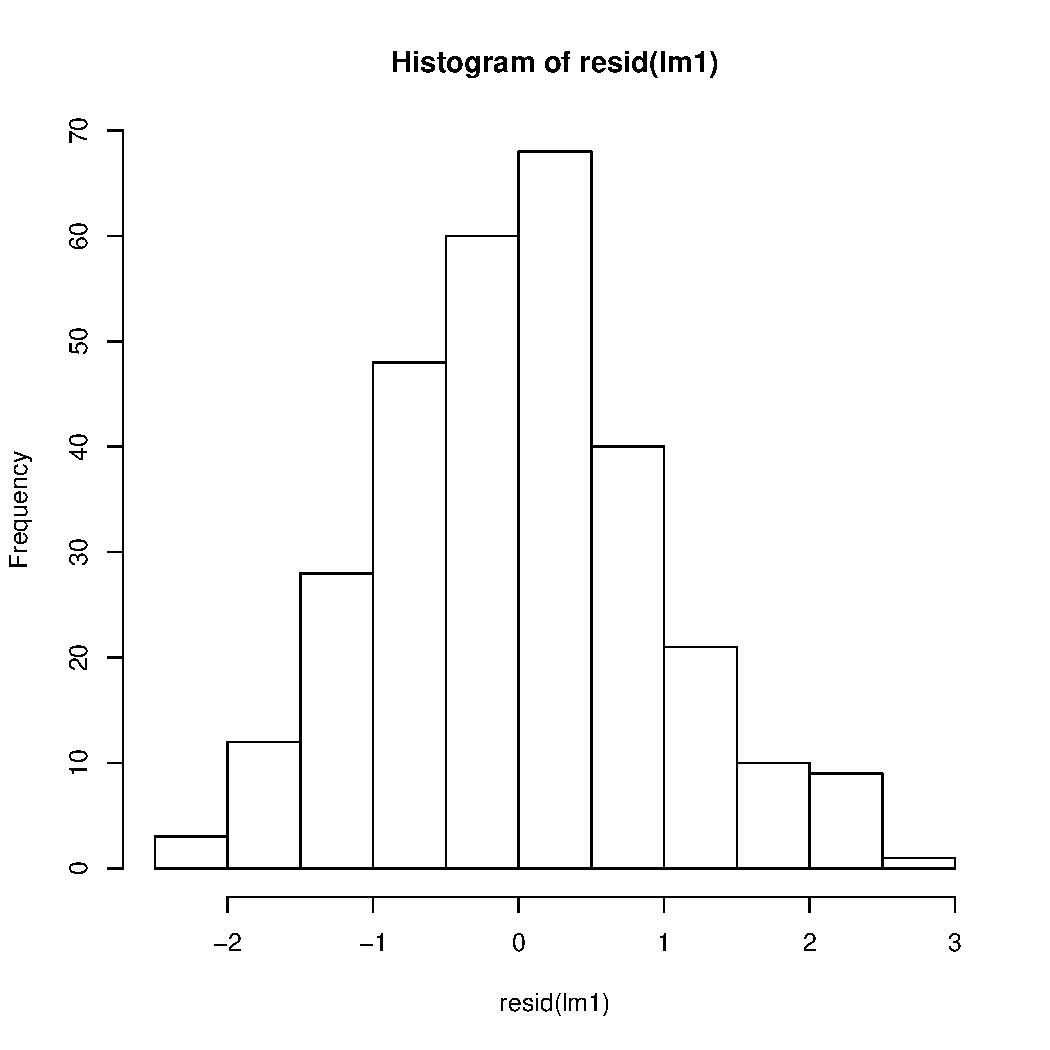
\includegraphics[width=\maxwidth]{figure/unnamed-chunk-3-1} 

\end{knitrout}

However, in our case, we have data about the missing variable that structure residuals, so we can see clearly that residuals are distributed with structure:
\begin{knitrout}
\definecolor{shadecolor}{rgb}{0.969, 0.969, 0.969}\color{fgcolor}\begin{kframe}
\begin{alltt}
\hlkwd{plot}\hlstd{(thorns}\hlopt{$}\hlstd{site,} \hlkwd{residuals}\hlstd{(model_0))}
\end{alltt}
\end{kframe}
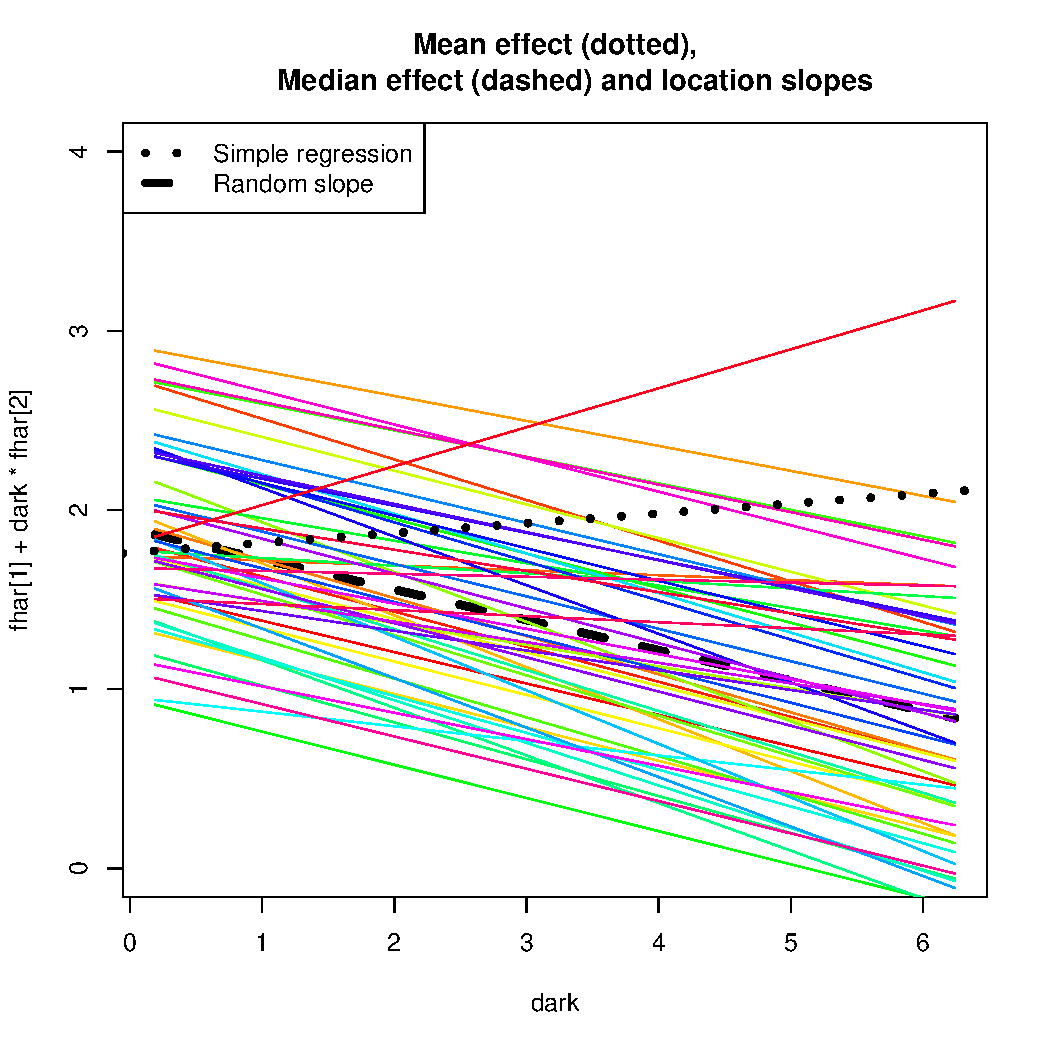
\includegraphics[width=\maxwidth]{figure/unnamed-chunk-4-1} 

\end{knitrout}

We can correct the problem by fititng site in the mode:
\begin{knitrout}
\definecolor{shadecolor}{rgb}{0.969, 0.969, 0.969}\color{fgcolor}\begin{kframe}
\begin{alltt}
\hlstd{model_1} \hlkwb{<-} \hlkwd{lm}\hlstd{(herbivory} \hlopt{~} \hlstd{thorndensity} \hlopt{+} \hlstd{site,} \hlkwc{data} \hlstd{= thorns)}
\hlkwd{summary}\hlstd{(model_1)}
\end{alltt}
\begin{verbatim}
## 
## Call:
## lm(formula = herbivory ~ thorndensity + site, data = thorns)
## 
## Residuals:
##     Min      1Q  Median      3Q     Max 
## -1.6877 -0.2889  0.0498  0.2492  1.3968 
## 
## Coefficients:
##              Estimate Std. Error t value Pr(>|t|)    
## (Intercept)     6.047      0.387   15.62  < 2e-16 ***
## thorndensity   -0.975      0.141   -6.90  6.0e-10 ***
## siteb           0.940      0.176    5.33  6.6e-07 ***
## sitec           1.996      0.215    9.30  5.8e-15 ***
## sited           2.971      0.281   10.56  < 2e-16 ***
## sitee           3.767      0.422    8.93  3.5e-14 ***
## ---
## Signif. codes:  0 '***' 0.001 '**' 0.01 '*' 0.05 '.' 0.1 ' ' 1
## 
## Residual standard error: 0.488 on 94 degrees of freedom
## Multiple R-squared:  0.615,	Adjusted R-squared:  0.595 
## F-statistic:   30 on 5 and 94 DF,  p-value: <2e-16
\end{verbatim}
\end{kframe}
\end{knitrout}

Now we see a negative relationship between thorn density and herbivory. 

That model corresponds to the plot below:
\begin{center}
  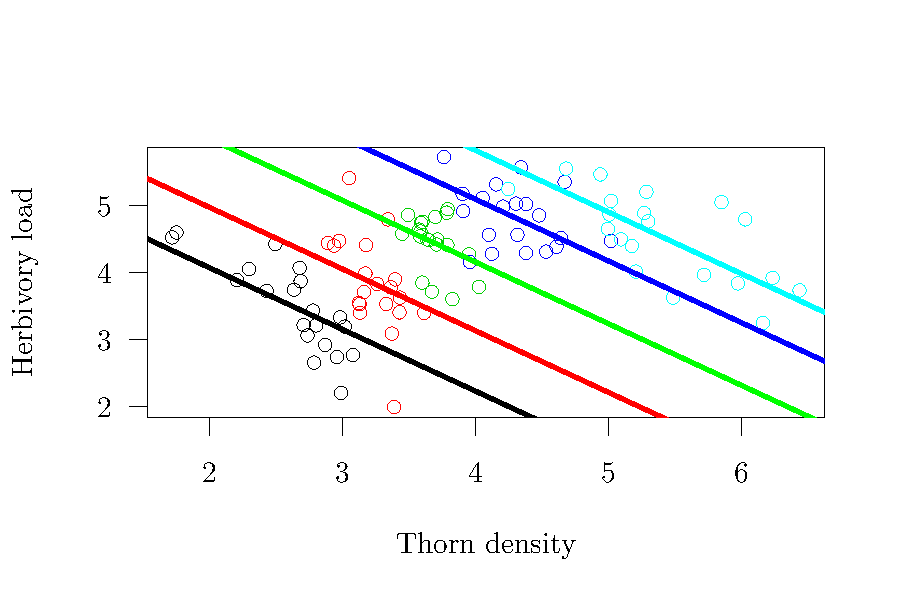
\includegraphics[width=0.8\textwidth]{figures/graph2-1.pdf}
\end{center}
We have 5 parallel regression lines, one for each site. Differences in the mean values within each sites are accounted for but we estimate the common slope across all sites.

The residuals of that model are more clearly without pattern:
\begin{knitrout}
\definecolor{shadecolor}{rgb}{0.969, 0.969, 0.969}\color{fgcolor}\begin{kframe}
\begin{alltt}
\hlkwd{plot}\hlstd{(}\hlkwd{residuals}\hlstd{(model_1))}
\end{alltt}
\end{kframe}
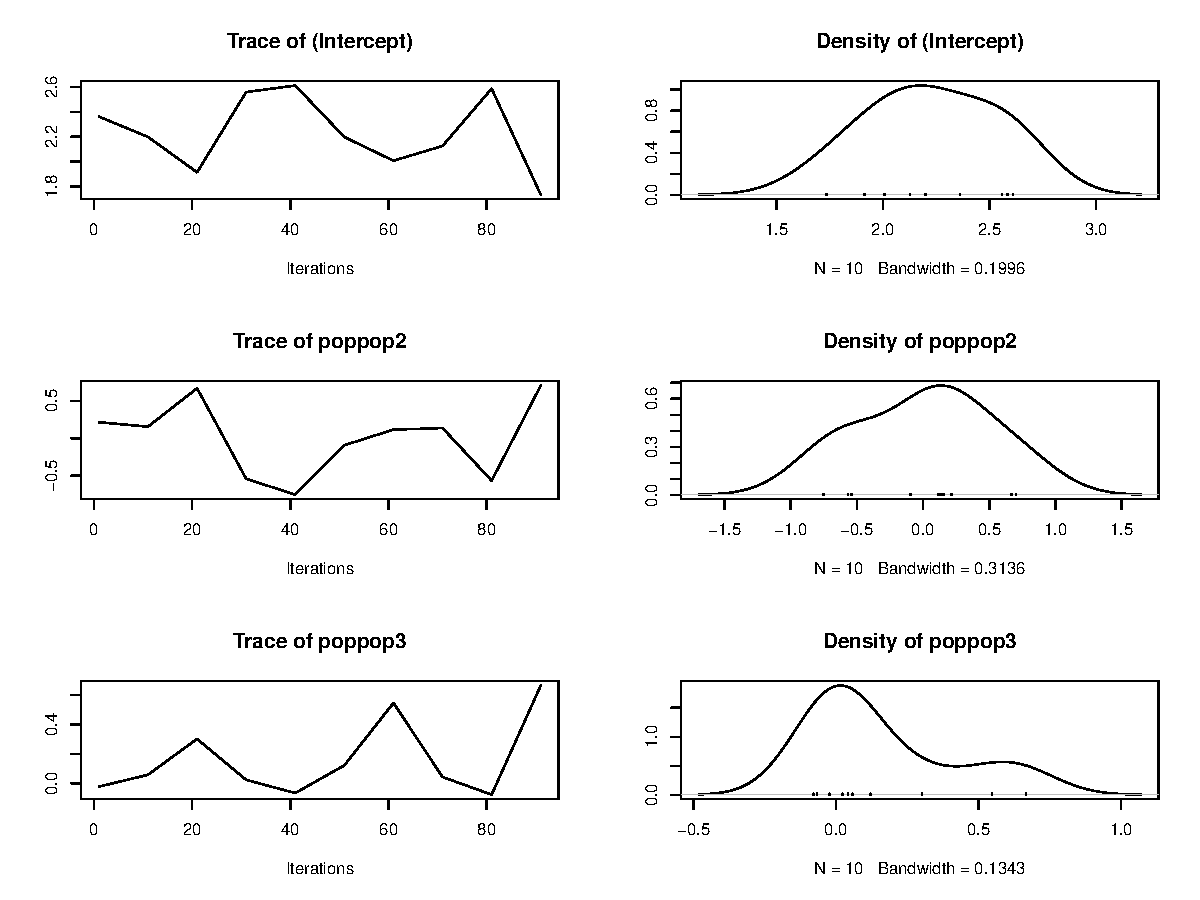
\includegraphics[width=\maxwidth]{figure/unnamed-chunk-6-1} 
\begin{kframe}\begin{alltt}
\hlkwd{plot}\hlstd{(thorns}\hlopt{$}\hlstd{site,} \hlkwd{residuals}\hlstd{(model_1))}
\end{alltt}
\end{kframe}
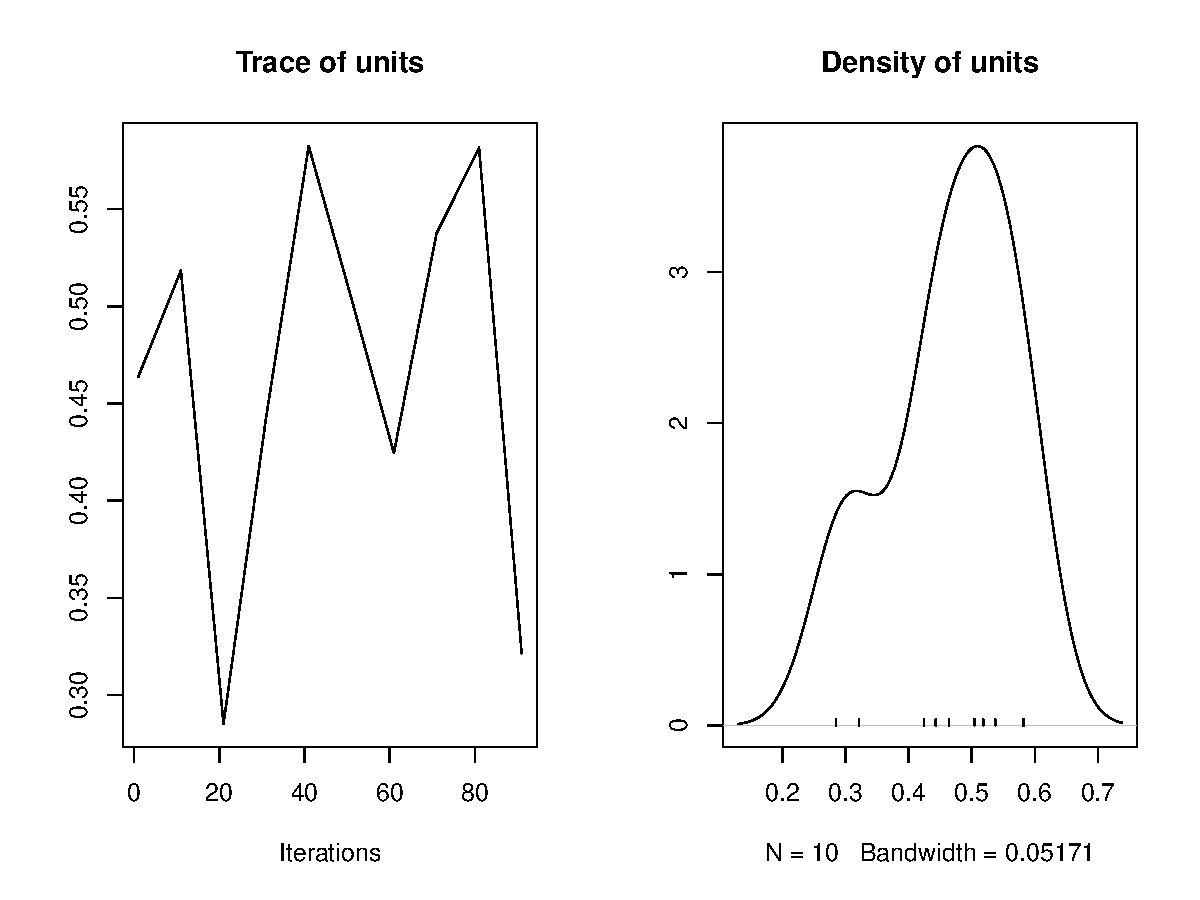
\includegraphics[width=\maxwidth]{figure/unnamed-chunk-6-2} 

\end{knitrout}


Note that in the summary of model\_1 we have 4 parameter estimates we did not really care about: the deviations of four site relative to the fifth site. It does not hurt to have them there, but we are not really interested in them because 1) we did not have questions about how sites vary in herbivory, 2) site is just a grouping factor and differences between sites are probably due to numerous processes we have not measured. Given our ignorance on what makes sites different, the values of site effects are essentially random; we fit site only to get a correct inference but do not learn much from the estimated effects of sites.

\section{Fitting random effects}

Now imagine a larger research setting where you would have collected data in 50 sites for a response variable and a predictor.


Check what happens if we approach the problem as in the thorn example:
\begin{knitrout}
\definecolor{shadecolor}{rgb}{0.969, 0.969, 0.969}\color{fgcolor}\begin{kframe}
\begin{alltt}
\hlstd{biggerdata} \hlkwb{<-} \hlkwd{read.csv}\hlstd{(}\hlstr{"Data/biggerdata.csv"}\hlstd{)}
\hlkwd{str}\hlstd{(biggerdata)}
\end{alltt}
\begin{verbatim}
## 'data.frame':	10000 obs. of  3 variables:
##  $ predictor: num  1.42 2.88 2.09 2.33 2.69 ...
##  $ response : num  1.594 3.016 0.964 2.356 2.379 ...
##  $ site     : Factor w/ 50 levels "s1","s10","s11",..: 17 35 45 12 25 17 43 40 49 23 ...
\end{verbatim}
\begin{alltt}
\hlstd{bdmodel} \hlkwb{<-} \hlkwd{lm}\hlstd{(response} \hlopt{~} \hlstd{predictor} \hlopt{+} \hlstd{site,} \hlkwc{data} \hlstd{= biggerdata)}
\hlkwd{summary}\hlstd{(bdmodel)}
\end{alltt}
\begin{verbatim}
## 
## Call:
## lm(formula = response ~ predictor + site, data = biggerdata)
## 
## Residuals:
##     Min      1Q  Median      3Q     Max 
## -1.9743 -0.3387  0.0037  0.3337  1.9768 
## 
## Coefficients:
##              Estimate Std. Error t value Pr(>|t|)    
## (Intercept)  1.972672   0.040038   49.27   <2e-16 ***
## predictor    0.212243   0.010043   21.13   <2e-16 ***
## sites10     -0.027050   0.049146   -0.55    0.582    
## sites11      0.024536   0.050654    0.48    0.628    
## sites12      0.016149   0.049828    0.32    0.746    
## sites13     -0.008957   0.049270   -0.18    0.856    
## sites14      0.039492   0.050439    0.78    0.434    
## sites15      0.037581   0.049764    0.76    0.450    
## sites16     -0.008394   0.049145   -0.17    0.864    
## sites17      0.007263   0.050031    0.15    0.885    
## sites18     -0.020866   0.050026   -0.42    0.677    
## sites19     -0.018773   0.049205   -0.38    0.703    
## sites2      -0.081374   0.049086   -1.66    0.097 .  
## sites20     -0.032109   0.050168   -0.64    0.522    
## sites21      0.029623   0.050301    0.59    0.556    
## sites22     -0.009032   0.050027   -0.18    0.857    
## sites23     -0.065420   0.052181   -1.25    0.210    
## sites24     -0.019260   0.047906   -0.40    0.688    
## sites25      0.030591   0.050583    0.60    0.545    
## sites26      0.025648   0.050440    0.51    0.611    
## sites27      0.008054   0.049763    0.16    0.871    
## sites28     -0.005345   0.049454   -0.11    0.914    
## sites29     -0.023777   0.050301   -0.47    0.636    
## sites3      -0.018559   0.049511   -0.37    0.708    
## sites30      0.027716   0.049895    0.56    0.579    
## sites31     -0.016783   0.049145   -0.34    0.733    
## sites32     -0.059918   0.048637   -1.23    0.218    
## sites33      0.009877   0.048745    0.20    0.839    
## sites34      0.017356   0.048912    0.35    0.723    
## sites35     -0.006882   0.049769   -0.14    0.890    
## sites36     -0.030452   0.050441   -0.60    0.546    
## sites37     -0.003812   0.049635   -0.08    0.939    
## sites38      0.054955   0.049207    1.12    0.264    
## sites39      0.016084   0.050026    0.32    0.748    
## sites4       0.021960   0.049385    0.44    0.657    
## sites40      0.018802   0.049448    0.38    0.704    
## sites41     -0.028651   0.049145   -0.58    0.560    
## sites42     -0.040484   0.049145   -0.82    0.410    
## sites43     -0.005169   0.050026   -0.10    0.918    
## sites44      0.011541   0.050438    0.23    0.819    
## sites45      0.033442   0.048206    0.69    0.488    
## sites46      0.015592   0.049898    0.31    0.755    
## sites47     -0.038314   0.049329   -0.78    0.437    
## sites48     -0.028233   0.048857   -0.58    0.563    
## sites49      0.011887   0.048208    0.25    0.805    
## sites5       0.021391   0.049828    0.43    0.668    
## sites50      0.000108   0.050094    0.00    0.998    
## sites6       0.006271   0.048799    0.13    0.898    
## sites7      -0.012073   0.049763   -0.24    0.808    
## sites8      -0.075520   0.049145   -1.54    0.124    
## sites9       0.048028   0.049968    0.96    0.336    
## ---
## Signif. codes:  0 '***' 0.001 '**' 0.01 '*' 0.05 '.' 0.1 ' ' 1
## 
## Residual standard error: 0.499 on 9949 degrees of freedom
## Multiple R-squared:  0.0463,	Adjusted R-squared:  0.0415 
## F-statistic: 9.66 on 50 and 9949 DF,  p-value: <2e-16
\end{verbatim}
\end{kframe}
\end{knitrout}

\begin{Exercise}[difficulty=1, title={Reading a summary in lme4}]
\begin{enumerate}
  \item Load the dataset "thorndata.txt" to fit a linear model of "herbivory" as a function of "thorndensity". What is the estimate for the slope?\\
  \item Add a random effect for site How does the estimate for the slope changes?\\
  \item How much variation is explained by differences among blocks? Is there a measure of uncertainty for this estimate?
\end{enumerate}
\end{Exercise}

\begin{Answer}
Part 1.
\begin{knitrout}
\definecolor{shadecolor}{rgb}{0.969, 0.969, 0.969}\color{fgcolor}\begin{kframe}
\begin{alltt}
\hlstd{thorns} \hlkwb{<-} \hlkwd{read.table}\hlstd{(}\hlstr{"Data/thorndata.txt"}\hlstd{,} \hlkwc{header} \hlstd{=} \hlnum{TRUE}\hlstd{)}
\end{alltt}


{\ttfamily\noindent\color{warningcolor}{\#\# Warning in file(file, "{}rt"{}): cannot open file 'Data/thorndata.txt': No such file or directory}}

{\ttfamily\noindent\bfseries\color{errorcolor}{\#\# Error in file(file, "{}rt"{}): cannot open the connection}}\begin{alltt}
\hlkwd{lm}\hlstd{(herbivory} \hlopt{~} \hlstd{thorndensity,} \hlkwc{data}\hlstd{=thorns)}
\end{alltt}
\begin{verbatim}
## 
## Call:
## lm(formula = herbivory ~ thorndensity, data = thorns)
## 
## Coefficients:
##  (Intercept)  thorndensity  
##        3.256         0.252
\end{verbatim}
\end{kframe}
\end{knitrout}
The slope is 0.2524.\\

Part 2.
\begin{knitrout}
\definecolor{shadecolor}{rgb}{0.969, 0.969, 0.969}\color{fgcolor}\begin{kframe}
\begin{alltt}
\hlkwd{library}\hlstd{(lme4)}
\end{alltt}


{\ttfamily\noindent\itshape\color{messagecolor}{\#\# Loading required package: Matrix}}\begin{alltt}
\hlkwd{summary}\hlstd{(}\hlkwd{lmer}\hlstd{(herbivory} \hlopt{~} \hlstd{thorndensity} \hlopt{+} \hlstd{(}\hlnum{1}\hlopt{|}\hlstd{site),} \hlkwc{data}\hlstd{=thorns))}
\end{alltt}
\begin{verbatim}
## Linear mixed model fit by REML ['lmerMod']
## Formula: herbivory ~ thorndensity + (1 | site)
##    Data: thorns
## 
## REML criterion at convergence: 165.3
## 
## Scaled residuals: 
##    Min     1Q Median     3Q    Max 
## -3.488 -0.606  0.109  0.523  2.873 
## 
## Random effects:
##  Groups   Name        Variance Std.Dev.
##  site     (Intercept) 2.129    1.459   
##  Residual             0.238    0.488   
## Number of obs: 100, groups:  site, 5
## 
## Fixed effects:
##              Estimate Std. Error t value
## (Intercept)     7.765      0.844    9.20
## thorndensity   -0.919      0.139   -6.63
## 
## Correlation of Fixed Effects:
##             (Intr)
## thorndensty -0.632
\end{verbatim}
\end{kframe}
\end{knitrout}
The slope is now NULL.\\

Part 3.
\begin{knitrout}
\definecolor{shadecolor}{rgb}{0.969, 0.969, 0.969}\color{fgcolor}\begin{kframe}
\begin{alltt}
\hlkwd{summary}\hlstd{(}\hlkwd{lmer}\hlstd{(herbivory} \hlopt{~} \hlstd{thorndensity} \hlopt{+} \hlstd{(}\hlnum{1}\hlopt{|}\hlstd{site),} \hlkwc{data}\hlstd{=thorns))}
\hlkwd{as.numeric}\hlstd{(}\hlkwd{VarCorr}\hlstd{(}\hlkwd{lmer}\hlstd{(herbivory} \hlopt{~} \hlstd{thorndensity} \hlopt{+} \hlstd{(}\hlnum{1}\hlopt{|}\hlstd{site),} \hlkwc{data}\hlstd{=thorns))}\hlopt{$}\hlstd{site)}
\end{alltt}
\end{kframe}
\end{knitrout}
The variance explained by block is  (careful, if you extract the standard deviation (Std.Dev.) you need to square it to obtain a variance.). There is no measure of uncertainty for the estimate of variance in block. In the \texttt{summmary} the \texttt{Std.Dev.} is simply the square root of \texttt{Variance}.
\end{Answer}



\subsection{Confidence intervals and Tests}
Sometimes random effects are part of the experimental design and are in the models only to control for confounding effects. But sometimes we care about their value or their statistical significance.


\begin{Exercise}[difficulty=1, title={CI for variance components in lme4}]
Use the function \texttt{confint} to estimate confidence intervals for the variance component for "site".
\end{Exercise}
\begin{Answer}
\begin{knitrout}
\definecolor{shadecolor}{rgb}{0.969, 0.969, 0.969}\color{fgcolor}\begin{kframe}
\begin{alltt}
\hlstd{lmm1} \hlkwb{<-} \hlkwd{lmer}\hlstd{(herbivory} \hlopt{~} \hlstd{thorndensity} \hlopt{+} \hlstd{(}\hlnum{1}\hlopt{|}\hlstd{site),} \hlkwc{data}\hlstd{=thorns)}
\hlstd{conf} \hlkwb{<-} \hlkwd{confint}\hlstd{(lmm1)}
\end{alltt}


{\ttfamily\noindent\itshape\color{messagecolor}{\#\# Computing profile confidence intervals ...}}\begin{alltt}
\hlstd{conf[}\hlnum{1}\hlstd{,]}\hlopt{^}\hlnum{2}
\end{alltt}
\begin{verbatim}
##  2.5 % 97.5 % 
## 0.5247 8.1932
\end{verbatim}
\end{kframe}
\end{knitrout}
\end{Answer}

\begin{tcolorbox}[colback=green!5,colframe=green!40!black,title=How does random effect formula work again?]
Random effect formula in lme4 and many other R-packages look like (1$|$group).

On the right-hand side of the pipe ($|$) is the variable that groups data points; for instance location, time, species\dots \\

On the left-hand side of the pipe is what varies according to grouping. In today's example we use only $1$, which stands for \textbf{intercept}. In other words we use random-intercept models. You can write other things on the left-hand side to define more complex models ("random interactions", "random regressions",\dots) but we will see that next time.

\end{tcolorbox}



\begin{tcolorbox}[colback=green!5,colframe=green!40!black,title=Fixed or random effect?]
When you want to include a categorical variable as a predictor in a model you can generally 
\begin{itemize}
\item First, if the predictor is a numerical variable (like size, temperature, number of species\dots) you will generally want a fixed effect, because the order and distance between values is likely meaningful. A random effect consider values as random "names" for grouping levels.
\item In general it does not change inference much. Random effects are slightly more efficient because the differences between grouping levels are assumed to come from a normal distribution, instead of being estimated independently from each other. 
\item A slightly lame but practical reason to use random effects: models output are cleaner with random effects because you get a single parameter estimate for a grouping variable modeled as a random effect, instead of a parameter estimate for each level of the grouping variable when modeled with a fixed effect.
\item Using a random effect instead of a fixed effect shifts the focus from the effect of each grouping level to variation among grouping levels. What is more interesting to you?
\item Often we use random effect to "correct" for some structure in the data that is not of interest. But random variance parameters can be of interest in themselves. For instance they can quantify genetic variation, individual repeatability, niche specialisation\dots if a variance parameter is of interest then estimate it using a random effect.
\item On the other hand, if you are very interested in how different a particular grouping level is from other levels, use fixed effects.
\item Be careful with random effects if the number of grouping levels is small. You definitely need at least 3, probably at least 5, maybe at least 10\dots With few grouping levels the fitting algorithm could have difficulties estimating the random variance, leading to unstable results (you may get different results from different algorithms) or the random variance being estimated to exactly zero.
\end{itemize}
\end{tcolorbox}

\section{}


\begin{Exercise}[difficulty=1, title={xxx}]

\end{Exercise}
\begin{Answer}

\end{Answer}

\section{More resources}


\href{http://bbolker.github.io/mixedmodels-misc/glmmFAQ.html}{Ben Bolker's GLMM FAQ is a gold mine if you need some technical details about mixed models (generalized or not).}

If you are going to do lots of mixed models consider subscribing to the mailing-list \href{https://stat.ethz.ch/mailman/listinfo/r-sig-mixed-models}{https://stat.ethz.ch/mailman/listinfo/r-sig-mixed-models}, ask questions or search the archive (anyway, Google is likely to directly send you to the archive).



\end{document}
